\documentclass{article}
\usepackage[margin=1in]{geometry}
\usepackage{mathtools, amsfonts, amsthm, amssymb, graphicx, listings, xcolor, pdfpages}


\definecolor{codegreen}{rgb}{0,0.6,0}
\definecolor{codegray}{rgb}{0.5,0.5,0.5}
\definecolor{codepurple}{rgb}{0.58,0,0.82}
\definecolor{backcolour}{rgb}{0.95,0.95,0.92}

\lstdefinestyle{mystyle}{
    backgroundcolor=\color{backcolour},   
    commentstyle=\color{codegreen},
    keywordstyle=\color{magenta},
    numberstyle=\tiny\color{codegray},
    stringstyle=\color{codepurple},
    basicstyle=\ttfamily\footnotesize,
    breakatwhitespace=false,         
    breaklines=true,                 
    captionpos=b,                    
    keepspaces=true,                 
    numbers=left,                    
    numbersep=5pt,                  
    showspaces=false,                
    showstringspaces=false,
    showtabs=false,                  
    tabsize=2
}

\lstset{style=mystyle}

\title{HW07}
\author{Sam Ly}

\begin{document}
\maketitle

\section*{Total points: }

\section*{Required Exercise 1 [4]}

Prove or disprove the following:

\begin{enumerate}
    \item {
        [1] There exists a pair of rational numbers \(a, b \in \mathbb{Q}\) with 
        \(a < b\) such that there is no \(c \in \mathbb{Q}\) with \(a < c < b\).

        \begin{proof}
            We see that for every pair of rational numbers \(a, b \in \mathbb{Q}\), 
            we can create a new rational number \(\frac{a+b}{2}\).

            Then, if \(a < b\), we see that \(a < \frac{a + b }{2} < b\). 
            Therefore, we have contradicted our original proposition, disproving the 
            original claim.
        \end{proof}

    }

    \item {
        [1] For all natural numbers \(n \in \mathbb{N}\), such that \(29 \nmid n\),
        \(2n^2 + 29\) is prime.

        \begin{proof}
            One counter-example to this claim is \(n = 29\). This is because when
            \(n = 29\), we get 
            \[2(29)^2 + 29\]
            \[29(2(29) + 1).\]
            This number is a product of 29 and \(2(29) + 1\), meaning it is not prime. 
            Therefore, we have disproven our original claim.
        \end{proof}
    }

    \item {
        [1] Let \(n\) be an integer, then \(10 \mid n\) if and only if \(100 \mid n^3\).

        \begin{proof}
            We begin by seeing that our proposition is equivalent to saying that 
            \(10 \mid n\) implies \(100 \mid n^3\) and \(100 \mid n^3\) implies \(10 \mid n\). 

            We continue by first proving \(10 \mid n \Rightarrow 100 \mid n^3\). 

            By using modular arithmetic, we see:
            \begin{align*}
                n &\equiv 0 \pmod{10}\\
                n^2 &\equiv 0 \pmod{100}\\
                n^3 &\equiv 0 \pmod{1000}.\\
            \end{align*}

            Since \(100 \equiv 0 \pmod{1000}\) and \(n^3 \equiv 0 \pmod{1000}\),
            \(n^3 \equiv 0 \pmod{100}\). So, \(100 \mid n^3\). 
            
            Therefore, \(n \mid 10 \Rightarrow n^3 \mid 100\).

            Now, to see that \(100 \mid n^3 \Rightarrow 10 \mid n\), we first 
            suppose \(100 \mid n^3\). Then, we see that \(4 \mid n^3\) and \(25 \mid n^3\).

            Thus, \(2 \mid n^3\) and \(2 \mid n\). Also, \(5 \mid n^3\) and \(5 \mid n\). 

            Since \(2 \mid n\) and \(5 \mid n\), \(10 \mid n\). 

            Therefore, \(10 \mid n\) if and only if \(100 \mid n^3\).
        \end{proof}
    }

    \item {
        [2] The square root of 2 is rational: \(\sqrt{2} \in \mathbb{Q }\).

        \begin{proof}
            We begin by assuming that \(\sqrt{2}\) is rational, and thus is can 
            be written in the form \(\frac{a }{b}\) for \(a, b \in \mathbb{Z}\)
            in lowest terms. Because \(\frac{a}{b}\) is in lowest terms, 
            they can not both be even. 

            Now, we see
            \begin{align*}
                \sqrt{2} &= \frac{a }{b } \\
                2 &= \frac{a^2}{b^2}\\
                b^2 &= \frac{a^2}{2}.\\
            \end{align*}

            Since \(b^2\) is an integer, \(a^2\) must be even. Since an odd number 
            squared is always odd, and an even number squared is always even, 
            \(a\) must be even. Thus, \(a = 2n\), for \(n \in \mathbb{Z}\).
            By substituting, we see 
            \begin{align*}
                b^2 &= \frac{(2n)^2}{2} = \frac{4n^2}{2} = 2n^2,\\
            \end{align*}

            meaning \(b^2\) is even and \(b\) is even. 

            We previously assumed that \(\frac{a }{b}\) was in lowest terms, and 
            thus can not both be even. Because we have arrived at a contradiction, 
            we can conclude that \(\sqrt{2}\) is not rational. 
        \end{proof}
    }
\end{enumerate}

\section*{Required Exercise 3 [2]}

One "stupid proof trick" is that quantified statements follow their own form of 
De Morgan's Laws. For example, when we say ``For all students \(s\) at CPP, \(s\) 
has a unique student ID.'' we can also say that ``There does not exist a student \(s\)
at CPP, where \(s\) has a preexisting student ID.''

This is one of the rare cases where the formal notation for quantified logical 
statements is useful because it lets us ``see'' the algebraic structure easier. 

Let \(P\) be some arbitrary logical statement, and \(\mathcal{U}\) be the universal set.
We see that:
\begin{align*}
    \forall x \in \mathcal{U}, P &\Leftrightarrow \neg (\exists x \in \mathcal{U}, \neg P)\\
    \exists x \in \mathcal{U}, P &\Leftrightarrow \neg (\forall x \in \mathcal{U}, \neg P).
\end{align*}

\section*{Required Exercise 4 [1]}
\begin{enumerate}
    \item {
        Done! I explicitly state that our proof will be inductive, and clarified 
        some structural elements. 
    }
    \item {
        I found the feedback very helpful. I like how simple and immediately 
        implementable the feedback is. 
    }
\end{enumerate}

\section*{Choice Exercise 10 [6]}

\begin{enumerate}
    \item {
        [1] Give examples of the following:
        \begin{itemize}
            \item {
                All 5 words (of length 3) that begin with \(a\) and begin with
                a non-trivial palindrome. 

                \[aaa, aab, aac, aba, aca.\]
            }

            \item{
                All 4 words that begin with \(a\) but do not begin with a non-trivial palindrome.

                \[abb, abc, acc, acb.\]
            }

            \item {
                A 7-letter word that does not begin with a non-trivial palindrome.

                \[abcabca.\]
            }
        \end{itemize}
    }

    \item {
        [1] perhaps my first original proof was that the number of 
        such words of length \(n\) was given by the formula
        \begin{align*}a(0) &= a(1) = 0, \text{ and}\\ a(n) &= 3a(n-1) + 3^{\lceil n/2 \rceil} - a(\lceil n/2 \rceil)\text{ for } n \geq 2 \text{,} \end{align*}
        where if \(x \in \mathbb{R}\) then the \emph{ceiling} of \(x\) is written 
        \(\lceil x \rceil\) and is the least ineger greater than or equal to \(x\).

        \begin{itemize}
            \item {
                Compute (by hand) \(\lceil 3.1415926 \rceil\), \(\lceil 3100 \rceil\), 
                and \(\lceil -9.19 \rceil\).

                \begin{align*}
                    \lceil 3.1415926 \rceil\ &= 4\\
                    \lceil 3100 \rceil\ &= 3100\\
                    \lceil -9.19 \rceil\ &= -9.
                \end{align*}
            }

            \item {
                Start a stopwatch, and try to write a computer program that will 
                compute \(a(26) = 1833980928771\). 

                \lstinputlisting[language=Python]{./code/ex10.py}
            }
        \end{itemize}
    }

    \item {
        [4] Recursion and induction are essentially the same idea. Use induction 
        to prove that the formula is correct.

        \begin{proof}
            We proceed with mathematical induction. We see that for our base cases 
            \(n = 0, 1\), there are no such strings that satisfy our condition 
            because there are no non-trivial palindromes of length 0 or 1. So, 
            \(a(0) = a(1) = 0\).

            For our inductive hypothesis, we assume
            \[a(n) = 3a(n-1) + 3^{\lceil n/2 \rceil} - a(\lceil n/2 \rceil) \text{ for } 2 \le n \le k. \]

            For \(n = k+1\),  we have
            \[a(k+1) = 3a(k) + 3^{\lceil k/2 \rceil} -a(\lceil k/2 \rceil).\]

            We arrive at this conclusion by seeing that when we increase our string 
            length by 1, we can:
            \begin{enumerate}
                \item append \(a\), \(b\), or \(c\) to the end of a previously valid string to create a new valid string.
                \item create a new palidrome of length \(k+1\) that begins with \(a\). 
            \end{enumerate}

            However, see that there are certain strings that are being counted twice
            between these two cases. For example, \(aaa \dots a\) can be created 
            from both case (a) and (b). 

            Specifically, the strings that are counted twice are the strings that 
            are both fully a palindrome, and contain a subpalindrome. The only 
            way for this to happen is if the first half of the string contains a palindrome. 

            Thus, our inductive step holds. Therefore, by induction, the n'th 
            term of our sequence is 
            \[a(n) = 3a(n-1) + 3^{\lceil n/2 \rceil} - a(\lceil n/2 \rceil) \text{ for } 2 \le n \le k. \]
        \end{proof}
    }
\end{enumerate}

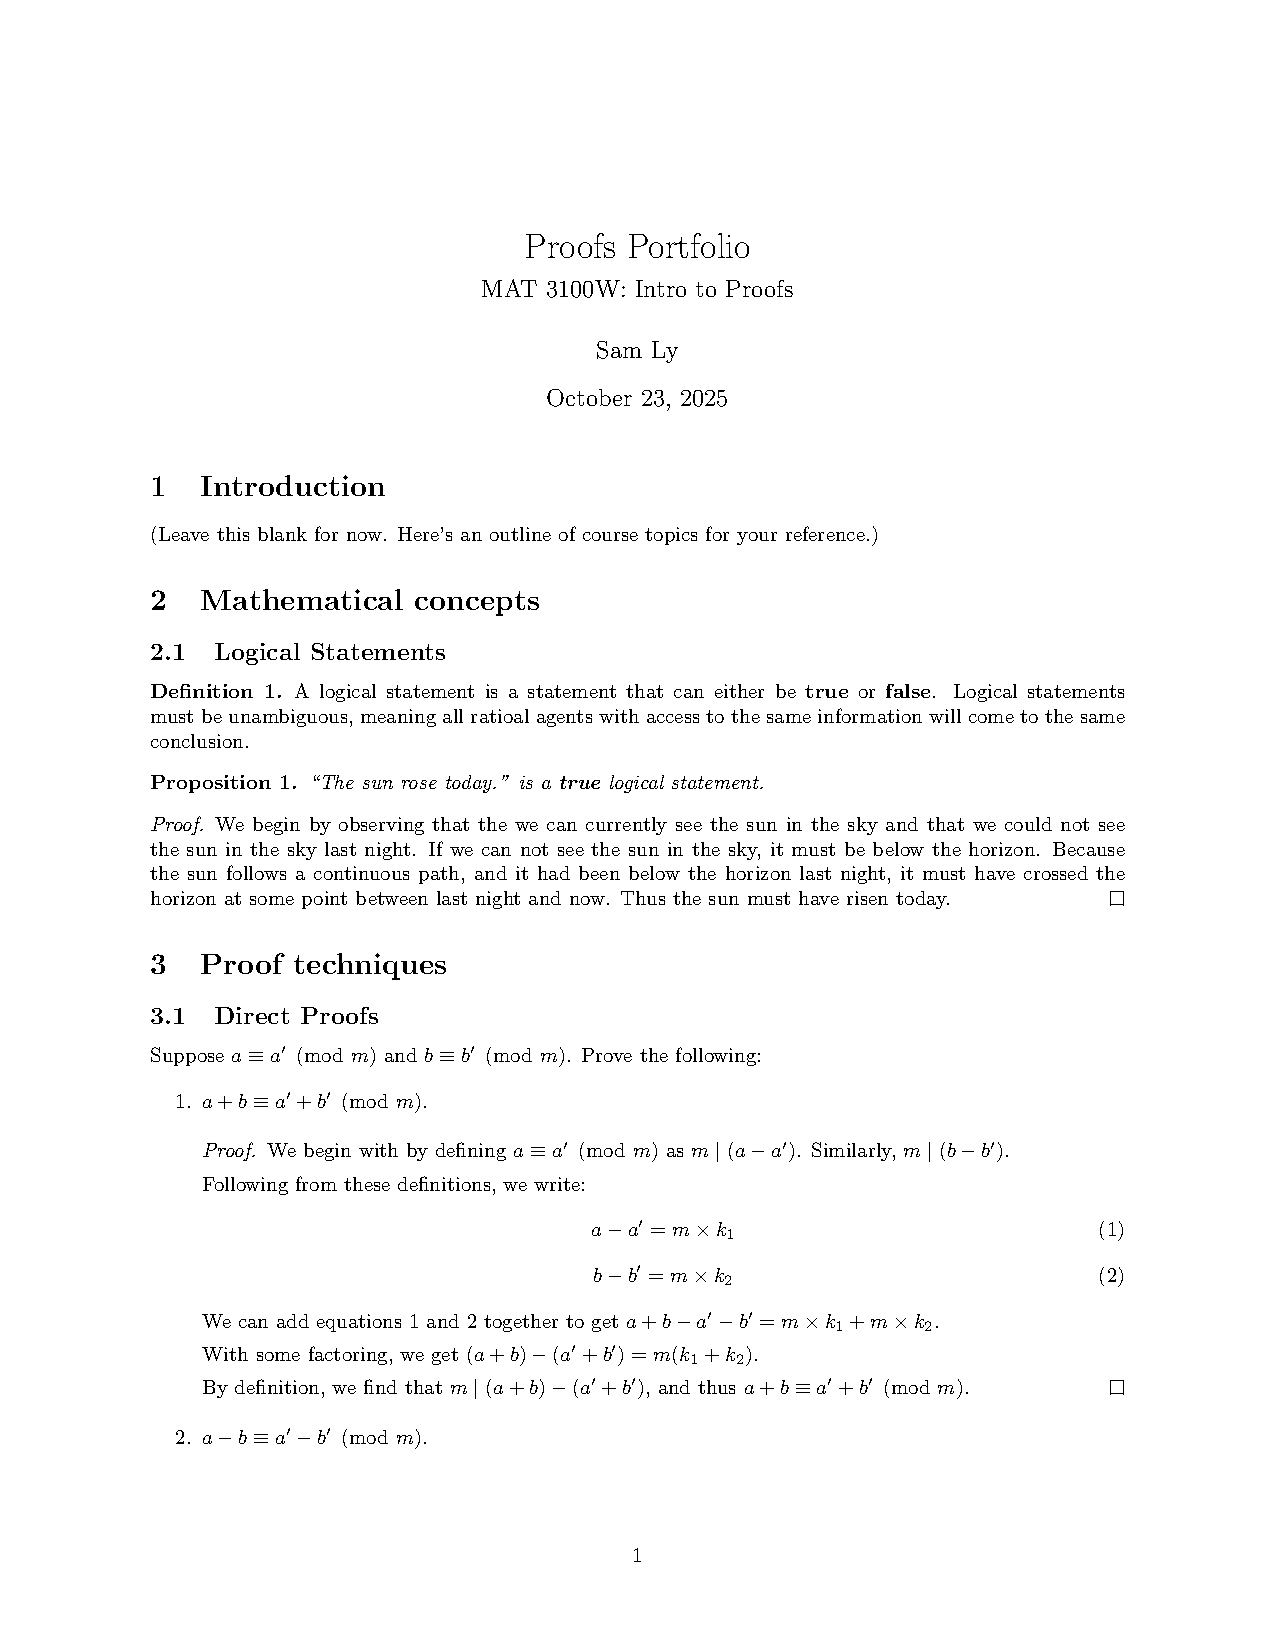
\includepdf[pages=-]{portfolio.pdf}
\end{document}